
\documentclass[
11pt,
titlepage,
a4paper,
ngerman,
captions=tableheading,
toc=bibliography,
%toc=listof,
numbers=noenddot
] {scrartcl}

\usepackage{ifpdf}
\usepackage[T1]{fontenc}
\usepackage[utf8]{inputenc}
\usepackage{microtype}
\usepackage{amsmath, amssymb, amstext}
%\usepackage{palatino}            % andere Schriftart
\usepackage[ngerman]{babel}       % Deutsch !
\usepackage[babel, german=quotes]{csquotes}
\usepackage{color}
\usepackage{graphicx}             % Bilder einbinden ermöglichen
\usepackage[obeyspaces]{url}                  % Besserew
\usepackage[textsize=small, textwidth=0.8in]{todonotes} % \todo noch zu tun
\usepackage{multirow}             % Zusammenfassen von Tabellenzellen
\usepackage{upgreek}              % nicht-kursive Griechische Buchstaben
\usepackage{textcomp}             % \textperthousand  (promille)
\usepackage{rotating}             % rotierte Information
\usepackage[format=plain, indention=1cm, scriptsize,font=sf, labelfont=bf, nooneline]{caption}
\usepackage{subfigure}%veraltet??
                                  % modif Bildunterschriften
\renewcommand{\captionfont}{\small \sffamily \slshape}
\renewcommand{\captionlabelfont}{\small \sffamily \slshape \bfseries   }

\usepackage[section]{placeins}
\usepackage{pdflscape}

%Einheiten
\usepackage[separate-uncertainty = true, locale=DE, alsoload=synchem]{siunitx}
\DeclareSIUnit{\ev}{\text{eV}}
\DeclareSIUnit{\u}{\text{u}}
\usepackage{units}

% Kontrolle der Seitenränder:
\usepackage[inner=3.5cm, outer=3cm, top=3cm, bottom=2cm, includehead, includefoot]{geometry}
% Besser nicht global als Standard setzen
%\clubpenalty=10000   % letzte Zeile einer Seite nicht erste Zeile eines Absatzes
%\widowpenalty=10000  % letzte Zeile eines Absatzes nicht erste Zeile einer Seite

% Eigene Kopf/Fußzeilen
\usepackage{fancyhdr}
\pagestyle{fancy}

% Standard:
\fancyhead[EL]{\thepage}
\fancyhead[ER]{\slshape \nouppercase{\leftmark}}
\fancyhead[OL]{\slshape \nouppercase{\leftmark}}
\fancyhead[OR]{\thepage}

% Fußzeile: Datum,  Seine X von Y, gut während des Schreibens:
\fancyfoot[EC, OC]{}%{\today{} $\ \ast\ast\ast\ $ Seite \thepage{}  von \pageref{LastPage}}

%neue Pakete
\usepackage{ae}
\usepackage{icomma}

\usepackage{hyperref}                            %macht anklickbare Links
\definecolor{LinkColor}{rgb}{0,0,0.75}           %dunkelblau
%\definecolor{LinkColor}{rgb}{0,0,0}             %schwarz

\hypersetup{
	pdftitle = {LaTeX-Vorlage},
	pdfsubject = {LaTeX-Vorlage},
	pdfkeywords = {LaTeX, Vorlage, Uni Wuppertal},
	pdfauthor = {Ich},
	bookmarksnumbered = true,
	bookmarksopen = false,
	colorlinks = false,
	hypertexnames = true,
	a4paper = true,
	colorlinks=true,%
	linkcolor=LinkColor,%
	citecolor=LinkColor,%
	filecolor=LinkColor,%
	menucolor=LinkColor,%
	urlcolor=LinkColor,
	breaklinks=true
}

%%%%Codedarstellung
% Custom colors
\usepackage{color}
\definecolor{deepblue}{rgb}{0,0,0.5}
\definecolor{deepred}{rgb}{0.6,0,0}
\definecolor{deepgreen}{rgb}{0,0.5,0}
\definecolor{bgcolor}{rgb}{0.95,0.95,0.95}

\usepackage{listings}

% Python style for highlighting
\newcommand\codestyle[1]{\lstset{
language=#1,
%basicstyle=\ttm,
otherkeywords={self},             % Add keywords here
%keywordstyle=\ttb\color{deepblue},
emph={MyClass,__init__,rld},          % Custom highlighting
emphstyle=\ttfamily\color{deepblue},    % Custom highlighting style
%stringstyle=\color{deepgreen},
%frame=tb,                         % Any extra options here
showstringspaces=false,            %
%%
keywordstyle=\bfseries\ttfamily\color{deepred},
identifierstyle=\ttfamily\color{black},
commentstyle=\color[RGB]{120, 191, 142},
stringstyle=\ttfamily\color[rgb]{0.81,0.17,0},%[RGB]{deepgreen},%[rgb]{0.627,0.126,0.941},{164,196,0}
basicstyle= \ttfamily\footnotesize\color[RGB]{49,102,145},
numberstyle=\scriptsize\color{black},
numbers=left,
stepnumber=1,
numbersep=10pt,
tabsize=2,
breaklines=true,
%prebreak = \raisebox{0ex}[0ex][0ex]{\ensuremath{\hookleftarrow}},
breakatwhitespace=false,
aboveskip={1.5\baselineskip},
  columns=fixed,
  upquote=true,
  extendedchars=true,
 frame=single,
rulecolor=\color{black},
backgroundcolor=\color{bgcolor},
}}


% External codefiles
\newcommand\codefile[3][,]{{
\codestyle{#2}
\lstinputlisting[#1]{#3}
}}

%%%%%

%%neue Kommandos
\newenvironment{changemargin}[2]{%
\begin{list}{}{%
\setlength{\topsep}{0pt}%
\setlength{\leftmargin}{#1}%
\setlength{\rightmargin}{#2}%
\setlength{\listparindent}{\parindent}%
\setlength{\itemindent}{\parindent}%
\setlength{\parsep}{\parskip}%
}%
\item[]}{\end{list}}

%Sachen nebeneinander packen + \parindent Fox
\newlength{\myParindent} %Zwischenspeicher für \parindent
\setlength{\myParindent}{\the\parindent}

\newcommand{\colw}{0.63\linewidth}% ändern mit \renewcommand
\newcommand{\colmarg}{-1.2cm}
\newcommand{\twocol}[2]{
\begin{changemargin}{\colmarg}{\colmarg + 0.5cm}
\begin{minipage}{\colw}
#1
\end{minipage}
\begin{minipage}{\linewidth - \colw}
#2
\end{minipage}
\end{changemargin}
}
\newcommand{\colcap}[1]{ %setzt irgendwie \parindent auf 0, kA was das noch alles verhaut.
\vspace{-1.6em}
\captionof{figure}{#1}
\vspace{1.4em}
\setlength{\parindent}{\the\myParindent} %daher alten Wert zurücksetzen
}
\newcommand{\resetcol}{
\renewcommand{\colmarg}{-1.2cm}
\renewcommand{\colw}{0.63\linewidth}
}

\newcommand{\ufrac}[3]{\SI{#1}{$\unit{\frac{#2}{#3}}$} }
\newcommand{\PM}{&\hspace{-0,3cm}$\pm$&\hspace{-0,3cm}}


\newcommand{\gq}[1]{\glqq #1\grqq ~} %German Quotes

%%%%%%%%%%%%%%%%%%%%%%%%%%%%%%%%%%%%%%%%%%%%%%%%%%%%%%%%%%%%%%%
\newcommand{\ttt}[1]{\verb|#1|} %Code Schrift
\DeclareUrlCommand\ttt{\texttt{\urlstyle{same}}}

% \newcommand{\codesize}[1]{ basicstyle= {\ttfamily#1\color[RGB]{49,102,145}} }
%\newcommand{\codesize}[1]{ \ttfamily#1\color[RGB]{49,102,145} }
\newcommand{\codesize}[1]{ \lstset{ basicstyle= {\ttfamily#1\color[RGB]{49,102,145}} } }

%\newenvironment{nrcode}{\lstlisting}}{\endlstlisting}
%\renewcommand\lstlistingname{Programm} %umbenennen??
%[numbers=left, frame=single]
\lstnewenvironment{nrcode}[1][,]{
\lstset{numbers=left, frame=single, #1}
}{}

\newenvironment{source}{\quote}{\endquote}

%%Inline-Code-Setup
\newcommand{\inlinecodestyle}[1]{
\codestyle{#1}
\lstset{numbers=none , frame=none, basicstyle= \ttfamily\small\color[RGB]{49,102,145}, aboveskip={0.5\baselineskip}}%, backgroundcolor=\color{white}}
}

\lstset{escapeinside={\#(*}{*)}} %fuer labels!
%%%%%%%%%%%%%%%%%%%%%%%%%%%%%%%%%%%%%%%%%%%%%%%%%%%%%%%%%%%%%%%

% Stil der Zitate und der Bibliographie
\usepackage[style=numeric, backend=biber, bibencoding=utf8, bibwarn=true, sorting=none
			%, hyperref=true, backref=true
]{biblatex}
\addbibresource{literatur.bib}



\title{ Einfacher Crosscompiler von Python nach C++ }
\subject{Programmierpraktikum}
\author{Felix Helsch \\ Julian Buchhorn}
\date{\today}

\publishers{\parbox[b][8cm]{\textwidth}{\centering \textbf{Betreuer}\\Dr. Holger Arndt}}

\usepackage[version=3]{mhchem}
\usepackage{rotating}
\usepackage{booktabs}

\newcommand{\cc}[1]{\multicolumn{1}{c}{#1}} %Cell-Center
\newcommand{\C}[2]{\multicolumn{#1}{|c|}{#2}} %multiCol-wall
\newcommand{\mc}[2]{\multicolumn{#1}{c}{#2}} %multicol

\inlinecodestyle{python}
\lstset{ escapeinside= {\#(*} {*)} }
\lstset{
 rangeprefix= \#\\*,
 includerangemarker= false,
 texcl= false, %??
}
%%%%%%%%%%%%%%%%%%%%%%%%%%%%%%%%%%%%%%%%%%%%%%%%%%%%%%%%%%%%%%%%%%%%%%
\begin{document}

\pagestyle{empty}
\maketitle
\tableofcontents

\lstlistoflistings
\listoffigures
%\clearpage
%\listoffigures
%\clearpage
%\listoftables
%\clearpage
%\lstlistoflistings

\clearpage
\pagestyle{fancy}
%%%%%%%%%%%%%%%%%%%%%%%%%%%%%%%%%%%%%%%%%%%%%%%%%%%%%%%%%%%%%%%%%%%%%%

\section{Einleitung}

Im Rahmen eines Programmierpraktikums an der Bergischen Universität Wuppertal haben wir einen Compiler von Python zu C++ geschrieben. Dabei ging es in erster Linie darum, zu verstehen wie ein Compiler funktioniert und nicht darum einen vollständigen Compiler zu schreiben.

Als vorläufiges Ziel hatten wir uns gesetzt ein einfaches Testprogramm mit grundlegenden Syntaxelementen zu übersetzen (vgl. Lst. \ref{pyprog}).

\codefile[caption= Python Testprogramm für den Compiler, label=pyprog]{python}{program.py}

Das Ziel haben wir erreicht. Unser Compiler kann in seinem momentanen Zustand das Python Programm übersetzen und liefert das C++ Programm in Listing \ref{cppprog}. Dabei mussten wir, wie erwartet, einige Annahmen über das Programm machen, um die Übersetzung zu vereinfachen.

\codefile[caption= Vom Compiler erzeugtes C++ Programm, label=cppprog]{c++}{program.cpp}


In den folgenden Kapiteln werden wir erklären wie man den Compiler verwenden kann, welche Programme benötigt werden und welche Features der Compiler im Moment unterstützt. Zum Schluss werden wir noch kurz auf die Struktur des Codes eingehen, den wir geschrieben haben.

Für eine detailliertere Erklärung verweisen wir auf die Bachelorarbeit von Felix Helsch, in welcher die Erstellung des Compilers fortgeführt wird.


%%%%%%%%%%%%%%%%%%%%%%%%%%%%%%%%%%%%%%%%%%%%%%%%%%%%%%%%%%%%%%%%%%%%%%

\section{Verwendung}

Um ein Python Programm nach C++ zu compilieren, muss man nur das Main-Programm \path{py2cpp.py} aufrufen und dabei den Namen des zu übersetzenden Programms als Kommandozeilenparameter angeben. Das heißt, dass zum Beispiel unser Testprogramm \ttt{program.py} mit dem folgenden Konsolenbefehl übersetzt werden kann:
\begin{lstlisting}
python py2cpp.py program.py
\end{lstlisting}
Dafür muss man allerdings die benötigten Programme installiert haben (s. Kapitel \ref{progs}) und beachten, dass das zu übersetzende Programm nur die momentan unterstützten Features enthält (s. Kapitel \ref{features}).
\enlargethispage{1cm}
%%%%%%%%%%%%%%%%%%%%%%%%%%%%%%%%%%%%%%%%%%%%%%%%%%%%%%%%%%%%%%%%%%%%%%

\section{Installation} \label{progs}

Zuerst muss man das Archiv mit den Compilerdateien herunterladen \cite{py2cpp} und an einer beliebigen Stelle auspacken.
Außerdem müssen Python und C++ installiert sein (siehe nächster Abschnitt).
Innerhalb dieses Verzeichnisses kann der Compiler dann wie beschrieben aufgerufen werden, wenn sich die zu übersetzende Datei ebenfalls im selben Verzeichnis befindet.
Sonst sollte man entsprechend den absoluten Pfad angeben.


\subsection{Benötigte Programme}

Folgende Programme werden zur Verwendung des Compilers in jedem Fall benötigt, jeweils in der angegebenen Version oder einer neueren:

\begin{itemize}
\item \ttt{Python} 2.7
\begin{itemize}
\item \ttt{pandas} 0.15.2
\end{itemize}

\item \ttt{C++} 11
\item \texttt{Python-Runtime für Antlr} 4.4
\end{itemize}
%%

Die \ttt{Python-Runtime} ist in dem Compiler Archiv schon enthalten, braucht also nicht extra installiert werden. Falls man sie doch runterladen möchte findet man sie in der entsprechenden Sektion der \ttt{Antlr} Website \cite{pyruntime}.

\ttt{pandas} ist ein Package für Python welches der Compiler ebenfalls benötigt. Da \ttt{pandas} wiederum von den Packages \ttt{numpy}, \ttt{python-dateutil} und \ttt{pytz} abhängt, müssen diese ebenfalls installiert werden. Falls man diese Installationen nicht alle manuell durchführen will, bietet es sich hier an einen Package Manager zu benutzten (für Python unter Windows z.B. \ttt{Anaconda}). Für eine detaillierte Installationanleitung verweisen wir auf die Website von \ttt{pandas}  \cite{pandas}.

\subsection{Optionale Programme}

Die nachfolgenden Programme werden prinzipiell nur benötigt, wenn man die Grammatik \ttt{py.g4} neukompillieren möchte:
\begin{itemize}
\item \ttt{Antlr} 4.4

\begin{itemize}
\item \ttt{Java} 1.6
\end{itemize}
\end{itemize}

\ttt{Antlr} bietet allerdings auch noch zusätzliche Funktionen für die sich eine Installation lohnen kann. Zum Beispiel kann \ttt{Antlr} auch grafische Ansichten des Parsetrees erzeugen (s. Abbildung \ref{g:tree}), welche sehr nützlich sind zur Fehlersuche, oder einfach nur um die Struktur des Parsetrees besser zu verstehen. Außerdem kann die Grammatik dann nicht nur für \ttt{Python} kompilliert werden, sondern auch für die anderen Sprachen welche \ttt{Antlr}  unterstützt.


Da \ttt{Antlr} in \ttt{Java} geschrieben ist, benötigt es auch eine \ttt{Java} Installation. Insgesamt ist die Installation von \ttt{Antlr} etwas aufwändiger (insbesondere unter Windows), weswegen wir dazu noch eine ausführlichere Anleitung verfasst haben, welche sich in Abschnitt \ref{antlr:I} des Anhangs befindet. Insbesondere für die Installation unter Linux wollen wir aber auch auf die Anleitung auf der \ttt{Antlr} Website verweisen \cite{antlr}.




%%%%%%%%%%%%%%%%%%%%%%%%%%%%%%%%%%%%%%%%%%%%%%%%%%%%%%%%%%%%%%%%%%%%%%

\section{Features} \label{features}

\subsection{Unterstützte Syntaxelemente}

Sowohl Lexer als auch Parser unterstützen prinzipiell alle Syntaxelemente von Python und funktionieren -- soweit getestet -- mit allen Python Programmen. %\todo{ richtig?? }

Bei der Codegenerierung werden bis jetzt nur die grundlegenden Syntaxelemente unterstützt: Schleifen, \ttt{if-elif-else} und \ttt{print} Statement. Von den Schleifen wird insbesondere auch die Python \ttt{for} Schleife je nachdem in eine Zähl- oder eine \ttt{foreach} Schleife übersetzt.

Für unser Testprogramm mussten wir, wie bereits erwähnt, einige Annahmen zur Vereinfachung treffen:

Alle Typdeklarationen haben wir als \ttt{double} angenommen. Dadurch ist das Übersetzen von einfachen Funktionen, wie in Zeile \ref{func} des Programms, möglich.

Insbesondere werden Variablendeklarationen noch nicht unterstützt. In Zeile \ref{array_decl} mussten wir deshalb einfach annehmen, dass ein \ttt{array} deklariert wird.

Außerdem benötigt das Python Programm noch einen \ttt{if __name__=="__main__"}-Block um beim Übersetzen zu erkennen, an welcher Stelle die \ttt{main} Funktion in C++ platziert werden soll.

 

\subsection{Fehlererkennung}

Der Compiler erkennt auch Fehler im zu kompilierenden Programm und gibt entsprechende Fehlermeldungen aus, die möglichst genau anzeigen, an welcher Stelle der Fehler aufgetreten ist und um welche Art von Fehler es sich handelt:

Ändert man z.B. Zeile \ref{par_err} des Testprogramms in
\begin{lstlisting}
for i in range(len(L):
\end{lstlisting}

erkennt der Lexer die fehlende Klammer und gibt folgende Meldung aus:
%\begin{lstlisting}[basicstyle= {\ttfamily\footnotesize\color[RGB]{49,102,145}}]
%[basicstyle= \codesize{\tiny}]
%\lstset{basicstyle= {\ttfamily\tiny\color[RGB]{49,102,145}}}
%\codesize{\footnotesize}
\begin{lstlisting}
CompilerError: 
---------------------------------------------------------------
 Lexer, File "program.py", line 18, col 19:
---------------------------------------------------------------
    L= [0]*10

    for i in range(len(L):
                  ^
  ERR: Missing Closer for  ( 
\end{lstlisting}

\clearpage

Ebenso werden falsche Operatoren erkannt, z.B. bei Änderung von Zeile \ref{op_err}:
\begin{lstlisting}
CompilerError: 
---------------------------------------------------------------
 Lexer, File "program.py", line 22, col 20:
---------------------------------------------------------------
            L[i]= f(i+1)
        else:
            L[i]+==1
                  ^
  ERR: Unknown operator +==
\end{lstlisting}

Und auch inkorrekte Einrückungen (Änderung in Zeile \ref{ind_err}):
\begin{lstlisting}
CompilerError: 
---------------------------------------------------------------
 Lexer, File "program.py", line 21, col 9:
---------------------------------------------------------------
        if i>3:
            L[i]= f(i+1)
         else:
        ^
  ERR: Dedentation to incorrect level  
\end{lstlisting}

Außerdem werden auch die Fehler automatisch weitergeleitet, welche der mit Antlr erstellte Parser findet. Antlr gibt typischerweise die betroffene Zeilen- und Spaltennummer an, sowie das nicht passende Zeichen und die Alternativen welche an dieser Stelle möglich wären. Zum Beispiel erzeugt eine Änderung von Zeile \ref{parse_err} in
\begin{lstlisting}
if i=7>3:
\end{lstlisting}
die Fehlermeldung
\begin{lstlisting}
line 20:12 mismatched input '=' expecting {'!=', '**', '>>', '^', '(', '>=', '<', '//', '<>', '+', '/', '<<', 'if', '<=', '&', 'is', '*', '.', ':', '[', '==', '|', '>', 'or', '%', 'in', 'and', 'not', '-', ':$blockbegin'}
\end{lstlisting}
da eine Zuweisung in Python immer ein eigenes Statement ist und keine Expression.\\


Natürlich ist die Fehlererkennung noch nicht vollständig. Das ist für diesen Crosscompiler aber auch nicht unbedingt nötig, da man normalerweise davon ausgehen kann, dass das zu übersetzende Python Programm korrekt ist.

Aber man kann erkennen, dass die Fehlererkennung mit unserem Compiler auch gut möglich ist und bei Bedarf könnte sie auch noch entsprechend erweitert werden.






\clearpage
%%%%%%%%%%%%%%%%%%%%%%%%%%%%%%%%%%%%%%%%%%%%%%%%%%%%%%%%%%%%%%%%%%%%%%

\section{Codestruktur}

Schließlich wollen wir in diesem Abschnitt noch kurz die Struktur unseres Codes erklären, damit man die Funktion des Compilers bei Interesse besser nachvollziehen kann.

In der \ttt{main} Datei \ttt{py2cpp.py} werden die verschiedenen Programmteile des Compilers aufgerufen:

\begin{description}

\item[\texttt{LexerLoop.lex(prog)}] Ruft den schleifenbasierten Lexer auf. Dieser Lexer hat den Vorteil, dass es einfacher ist an bestimmten Stellen Fehlermeldungen einzufügen, da das Programm Buchstabe für Buchstabe durchlaufen wird.

 Der Lexer welchen wir eigentlich verwendet haben, basiert auf regulären Ausdrücken und wird als Teil von \ttt{space2braces(prog)} aufgerufen.
 
\item[\ttt{space2braces(prog)}] Lext das Programm mit regulären Audrücken, findet aus der Einrückung Blockanfang und -ende herraus und fügt entsprechende Tokens ein (ebenso für Statement Ende). Gibt den Namen der so generierten Programmdatei zurück.

\item[\ttt{compile_grammar()}] Damit kann das Neukompilieren der Antlr Grammatik \ttt{py.g4} optional  auch direkt aus dem  Wrapper gestartet werden. Beim kompilieren zu Python erzeugt Antlr die Dateien: \ttt{pyLexer.py}, \ttt{pyListener.py}, \ttt{pyParser.py}, \ttt{py.tokens} und  \ttt{pyLexer.tokens}.

\item[\ttt{pytree(prog_)}] Parst das umgewandelte Programm \ttt{prog_} mit dem aus der Antlr Grammatik generierten Parser. Anschließend wird der Parsetree mit dem Listener von Antlr durchlaufen und in unserem eigenen Parsetree gespeichert, welcher dann zurückgegeben wird.


\item[\ttt{AST.tofile(prog.replace('.py', '.cpp'))}] Durchläuft den Parsetree, wandelt die Python Syntax in C++ Syntax um und speichert das Ergebnis unter demselben Namen wie das Ausgangsprogramm, nur mit Endung \ttt{cpp} statt \ttt{py}.

\end{description}

\ttt{space2braces(...)} ist definiert in \ttt{space2braces.py} und befindet sich im Ordner \ttt{pylex} zusammen mit den restlichen Dateien, welche für den Lexer benötigt werden

\ttt{pytree(...)} ist definiert in \ttt{antlr2py.py} und ruft \ttt{parsetree.py} auf, wo die Datenstruktur für den Parsetree definiert ist, welche die Methode \ttt{tofile} besitzt. In \ttt{parsetree.py} befinden sich im Moment außerdem auch die Visitor Methoden für den Parsetree, das heißt dort findet die eigentliche Codegenerierung statt.

%%%%%%%%%%%%%%%%%%%%%%%%%%%%%%%%%%%%%%%%%%%%%%%%%%%%%%%%%%%%%%%%%%%%%%

\appendix
\newpage


%%%%%%%%%%%%%%%%%%%%%%%%%%%%%%%%%%%%%%%%%%%%%%%%%%%%%%%%%%%%%%%%%%%%%%


\section{Installation und Verwendung von Antlr} 

\ttt{Antlr} ist prinzipiell ein Parser-Generator mit ähnlicher Syntax wie \ttt{Yacc} oder \ttt{Bison}. Der hauptsächliche Unterschied liegt darin, dass im Gegensatz zu \ttt{Yacc} ein recursiv-descent Parser erzeugt wird. Daraus ergibt sich der Vorteil, dass \ttt{Antlr} bessere Fehlermeldungen erzeugen kann. Ein Nachteil ist, dass keine indirekte Linksrekursion möglich ist.

Für eine Erklärung der Syntax verweisen wir auf die \ttt{Antlr} Homepage \cite{antlrH}, in diesem Kapitel werden nur die Installation beschrieben und die benötigten Kommandozeilenaufrufe für \ttt{Antlr} bzw. den erzeugten Parser.

\subsection{Installation} \label{antlr:I}

Im folgenden geben wir die einzelnen Installationsschritte für Antlr an:

\begin{enumerate}

\item Installation des Java Development Kit (SDK/JDK) in der Version 1.6 oder höher

\item Download \ttt{Complete ANTLR 4.4 Java binaries jar} (oder neuer) \cite{antlrD}



\item Kopieren der heruntergeladenen Java-Bibliothek in den \ttt{jre/lib/ext} Ordner des JDK (zum Beispiel: \verb|C:\Program Files (x86)\Java\jdk1.8.0_25\jre\lib\ext| \\ bzw. unter Linux: \verb|/usr/lib64/jdk1.8.0_25/jre/lib/ext/|)


\item Hinzufügen der \ttt{.jar} Datei zum Klassenpfad \todo{ jre vs jdk? => geht beides!}

\emph{Optional}: Alias Einträge für Antlr und das Ausführen des Parsers anlegen

\end{enumerate}

Den Path- und die Aliaseinträge kann man unter Windows zum Beispiel vornehmen in dem man die folgenden Zeilen zum Powershell Profil hinzufügt: \todo {execution policy}

\begin{nrcode}[caption= Path- und Aliaseinträge für Antlr am Beispiel von Powershell unter Windows]
$env:Path+= ";C:\Program Files\Java\jre8\lib\ext\antlr-4.5-complete.jar"

function antlr {java org.antlr.v4.Tool $args}
function grun {java org.antlr.v4.runtime.misc.TestRig $args}
\end{nrcode}
%$ %fix highliting




\subsection{Rekompilieren und grafische Syntaxtree-Ansicht}

Nachdem man Antlr wie im vorherigen Kapitel beschrieben installiert hat, kann man eine Grammatik kompilieren indem man Antlr mit dem jeweiligen Grammatiknamen aufruft, dass heißt für unsere Pythongrammatik \ttt{py.g4}:
\begin{lstlisting}
antlr py.g4
\end{lstlisting}
Standardmäßig wird aus der Grammatik nun ein Parser in Java generiert. Möchte man den Parser in einer anderen Sprache verwenden, kann man die Grammatik auch in eine andere Zielsprache kompilieren, sofern sie von Antlr unterstützt wird. Für Python 2 zum Beispiel ändert man den Aufruf dafür folgendermaßen ab: \enlargethispage{1cm}
\begin{lstlisting}
antlr py.g4 -Dlanguage=Python2
\end{lstlisting}



Mit dem Java Parser kann man auch noch weitere Funktionen von Antlr nutzen, so ist es dann z.B. möglich beim Parsen eine grafische Darstellung des Parsetrees anzuzeigen, wie in Abbildung \ref{g:tree}. Der dargestellte Parsetree zeigt eine Funktion aus unserem Beispielprogramm.

Zur Erzeugung des Parsetrees kompiliert man zuerst die Grammatik nach Java, übersetzt dann die Java Dateien in ausführbare Dateien und wendet schließlich den Parser auf das gewünschte Programm an. Das heißt für unsere Grammatik, angewendet auf unser Beispielprogramm, verwendet man die folgenden Aufrufe:
\begin{lstlisting}
antlr py.g4
javac py*.java
grun py prog -gui "program.py"
\end{lstlisting}
Das zweite Argument  beim Ausführen des Parsers ist die Startregel der Grammatik (hier \ttt{prog}).
\begin{center}
 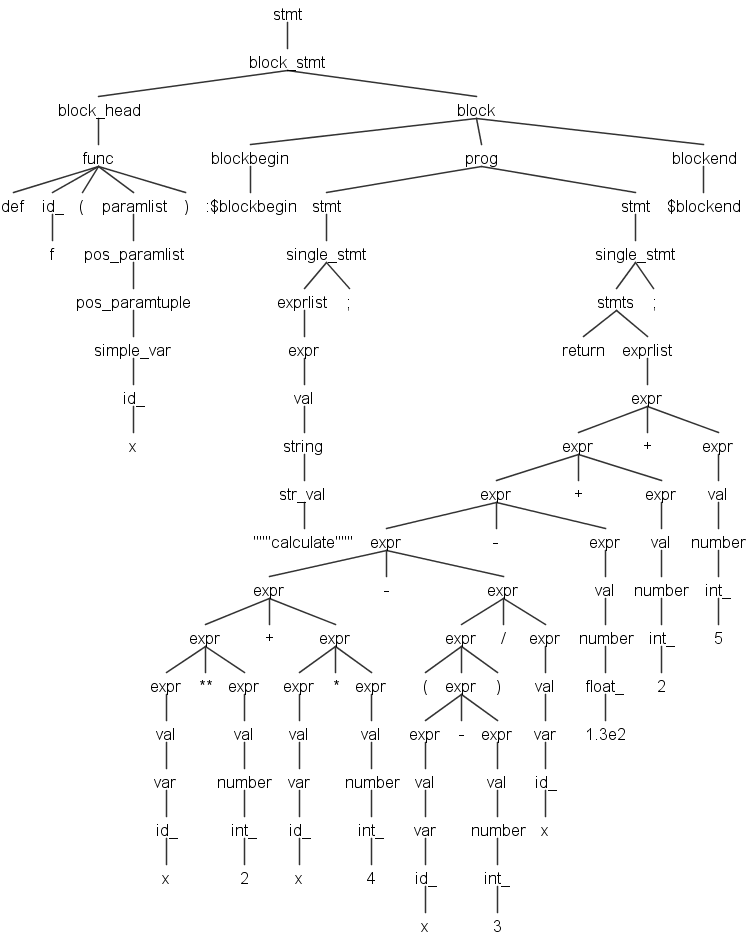
\includegraphics[width=0.8\linewidth]{Bilder/program_func_parse_tree2.png}
 \captionof{figure}{ Beispiel$  $ Parsetree } \label{g:tree}
\end{center}



\clearpage
\nocite{*}
\printbibliography

\end{document}
%%%%%%%%%%%%%%%%%%%%%%%%%%%%%%%%%%%%%%%%%%%%%%%%%%%%%%%%%%%%%%%%%%%%%%%%

\subsubsection*{Code Schrift}
Text mit \ttt{Code} \ttt{Schrift} .

\subsubsection*{Inline Code}
\begin{lstlisting}[caption=CAP]
inline code test
\end{lstlisting}

\vspace{4ex}
\subsubsection*{Numerierter Inline Code}
\begin{nrcode}[caption=CCC, label=pynr, linerange={a-c, d-e}]
import math
#\*a
2
nr code test #(*\label{txtline}*)
4
5
#\*b
6
7
#\*c
8
9
#\*d
10
11
#\*e
12
\end{nrcode}

Referenz für Code \ref{pynr} Zeile \ref{txtline}.

Referenz für Code \ref{pycode} Zeile \ref{test_arith}.